\section{Azure infrastruktúra áttekintése}
A Bus4U rendszer a Microsoft Azure felhőalapú platformján került telepítésre. Az Azure szolgáltatások skálázhatóságot és megbízhatóságot biztosítanak a rendszer számára. A telepítéshez az alábbi főbb szolgáltatásokat használtam:
\begin{itemize}
    \item \textbf{Azure Virtual Machines (VM)}: A szerver hosztolása.
    \item \textbf{Azure Database for PostgreSQL}: Az adatbázis-szolgáltatás biztosítása.
\end{itemize}

\section{Domain konfiguráció}
A rendszer az \textbf{api.bus4u.online} domainen érhető el, amelyet a Cloudflare platformján konfiguráltam. A domain hozzárendelése során a virtuális gép (VM) IP címét használtam. A következő beállításokat végeztem el:
\begin{itemize}
    \item \textbf{DNS beállítások}: A Cloudflare-en elvégeztem a domain névhez tartozó A és CNAME rekordok konfigurálását.
    \item \textbf{SSL tanúsítványok}: A HTTPS alapú kapcsolat biztonságának érdekében a Cloudflare szolgáltatásait alkalmazzuk, amelyek védelmet nyújtanak a felhasználók számára.
\end{itemize}


\section{Adatbázis telepítése és konfigurációja}
A rendszer adatbázisa egy \textbf{Azure Database for PostgreSQL} szolgáltatáson keresztül került telepítésre, amely lehetővé teszi az adatbázis automatikus méretezését és a folyamatos biztonsági mentések készítését. A következő beállításokat alkalmaztuk:
\begin{itemize}
    \item \textbf{Titkosított kapcsolatok}: A PostgreSQL adatbázis SSL tanúsítványokat használ a biztonságos kommunikációhoz.
    \item \textbf{Backup és recovery}: Automatikus biztonsági mentések kerülnek tárolásra az adatvesztés elkerülése érdekében.
\end{itemize}

\section{Szerver telepítése}
A szerver az \textbf{Azure Virtual Machines} szolgáltatásban került telepítésre, ahol a Ruby on Rails alapú API-t futtatjuk. A telepítés során a következő lépéseket hajtottuk végre:
\begin{itemize}
    \item \textbf{Környezeti változók beállítása}: A szükséges konfigurációs változók (pl. adatbázis kapcsolatok) a Ruby on Rails beépített credentials funkciójában lettek biztonságosan tárolva és kezelve.
    \item \textbf{Verziókezelés}: Az \textbf{asdf} verziókezelő használatával a Ruby és egyéb nyelvek verzióit könnyen kezelhetjük, ami megkönnyíti a fejlesztési környezet fenntartását.
    \item \textbf{CI/CD pipeline}: Az alkalmazás automatikus telepítése és frissítése a GitHub Actions integrációjával valósult meg.
\end{itemize}

\begin{figure}[H]
    \centering
    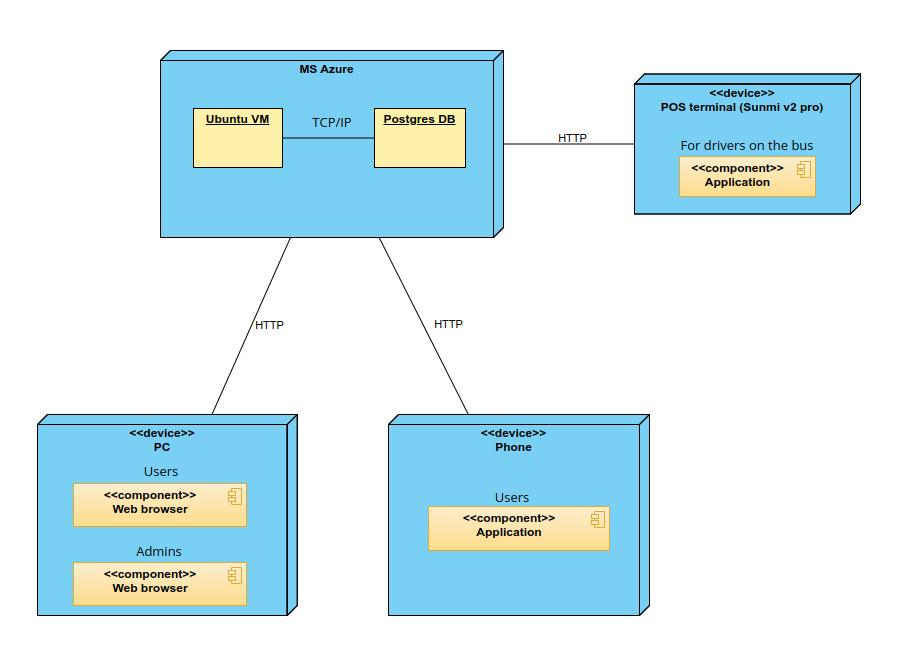
\includegraphics[width=\textwidth]{figures/deployment.jpg}
    \caption{Telepítési diagram}
    \label{fig:deployment-diagram}
  \end{figure}